\graphicspath{{./figures/}}
\title{static analysis}
\date{}
\begin{document}
\begin{frame}
    \titlepage
\end{frame}


\makeatletter
\newenvironment<>{btHighlight}[1][]
{\begin{onlyenv}#2\begingroup\tikzset{bt@Highlight@par/.style={#1}}\begin{lrbox}{\@tempboxa}}
{\end{lrbox}\bt@HL@box[bt@Highlight@par]{\@tempboxa}\endgroup\end{onlyenv}}

\newcommand<>\btHL[1][]{%
  \only#2{\begin{btHighlight}[#1]\bgroup\aftergroup\bt@HL@endenv}%
}
\def\bt@HL@endenv{%
  \end{btHighlight}%   
  \egroup %
}
\tikzset{
    btHLbox/.style={
        fill=red!30,outer sep=0pt,inner xsep=1pt, inner ysep=0pt, rounded corners=3pt
    },
}
\newcommand{\bt@HL@box}[2][]{%
  \tikz[#1]{%
    \pgfpathrectangle{\pgfpoint{1pt}{0pt}}{\pgfpoint{\wd #2}{\ht #2}}%
    \pgfusepath{use as bounding box}%
    \node[text width={},draw=none,anchor=base west, btHLbox, minimum height=\ht\strutbox+1pt,#1]{\raisebox{1pt}{\strut}\strut\usebox{#2}};
  }%
}

\lst@CCPutMacro
    \lst@ProcessOther {"2A}{%
      \lst@ttfamily 
         {\raisebox{2pt}{*}}% used with ttfamily
         {\raisebox{2pt}{*}}}% used with other fonts
    \@empty\z@\@empty

\lstdefinelanguage
   [x8664gas]{Assembler}     % add a "x64" dialect of Assembler
   [x86masm]{Assembler} % based on the "x86masm" dialect
   % with these extra keywords:
   {morekeywords={CDQE,CQO,CMPSQ,CMPXCHG16B,JRCXZ,LODSQ,MOVSXD,%
                  POPFQ,PUSHFQ,SCASQ,STOSQ,IRETQ,RDTSCP,SWAPGS,.TEXT,.STRING,.ASCIZ,%
                  BEQ,LW,SW,LB,SB,ADDIU,J,BEQZ,BNEZ,BNE,%
                  MOVUPD,MULPD,MOVSD,MULSD,%
                  SHLADD,MOV,CMP.LT,TBIT.NZ,BR.RET.SPTK.MANY,%
                  ADDQ,POPQ,PUSHQ,RRMOVQ,MRMOVQ,RMMOVQ,IRMOVQ,%
                  <-,LL,SC,ADDI,ADDL,VMOVDQA,ADDQ,CMPL,JB,JBE,MOVL,CLTQ,%
                  MOVW,PUSHW,MOV,ADD,SUB,INT,PUSH,MOV,ADD,REP,MOVSB,%
                  TESTQ,CMPQ,MOVL,MOVQ,ADDQ,JMPQ,XORQ,%
                  LEAQ,LEAL,LEA,RETQ,RET,POPL,POPW,PUSHL,PUSHW,%
                  LEAW,%
                  SUBQ,SYSCALL,.ASCII,CALLQ,MOVSLQ,JMP,ANDQ,SHRQ,MOVB,INCQ,TESTL,XORL,%
                  SHRL,LEAL,SARL,SUBL,IMULL,IMULQ,MOVDQU,PADDD,XORL,%
                  MOVZBL,MOVZB,SHRB,SRAL,SHRL,ANDL,%
                  CMOVNS,SRAL,SRAQ,MOVZBW,MOVZBQ,%
                  PADDW,PADDQ,MODUPS,MOVAPD,%
                  MOVL,RET,.GLOBL,%
		  PAUSE,LFENCE,JMP,%
                  },
    deletekeywords={eax,ebx,sp,si,cx,di,ds,cs,es,fs,dx,ax,bx,al,esi,ebp,ecx,rip,eip,edx,edi,rdi,esp},
    deletekeywords=[2]{size},
    alsoletter={\%},
    alsoother={()},
    emphstyle={\color{violet!50!black}},
    emph={\%rax,\%rbx,\%rcx,\%rdx,\%r8,\%r9,\%r10,\%r11,\%r12,\%r13,\%r14,\%r15,\%eax,\%ebx,\%sp,\%si,\%cx,\%di,\%ds,\%cs,\%es,\%fs,\%dx,\%ax,\%bx,\%al,\%esi,\%ebp,\%ecx,\%rip,\%eip,\%edx,\%edi,\%rdi,\%esp,\%rsp},
    %moreemph={eax,ebx,sp,si,cx,di,ds,cs,es,fs,dx,ax,bx,al,esi,ebp,ecx,rip,eip,edx,edi,rdi,esp},
    morecomment=[l]{\#},
    morecomment=[l]{\/\/},
    morecomment=[s]{/*}{*/},
    sensitive=false,
    keepspaces=true} % et

\lstalias[]{myasm}[x8664gas]{Assembler}

\lstdefinelanguage{JavaScript}{
  keywords={typeof, new, true, false, catch, function, return, null, catch, switch, var, if, in, while, do, else, case, break},
  ndkeywords={class, export, boolean, throw, implements, import, this},
  sensitive=false,
  comment=[l]{//},
  morecomment=[s]{/*}{*/},
  morestring=[b]',
  morestring=[b]"
}

\newcommand{\keywordstyle}{\sourcecodeprolight\bfseries\color{blue!30!black}}
\newcommand{\stringstyle}{\color{blue!20!black}\ttfamily}

\lstset{
    language=C,
    basicstyle=\sourcecodepro\EmptyMapping,
    escapechar=`,
    keywordstyle=\keywordstyle\EmptyMapping,
    identifierstyle=\sourcecodepro\EmptyMapping,
    numberstyle=\small\color{black!70},
    commentstyle=\color{red!60!black}\ttfamily\itshape,
    stringstyle=\color{blue!20!black}\ttfamily,
    ndkeywordstyle=\bfseries\color{blue!30!black},
    upquote=true,
}



\lstdefinestyle{medium}{
    basicstyle=\sourcecodepro\EmptyMapping\fontsize{12}{13}\selectfont,
    keywordstyle=\sourcecodepro\EmptyMapping\fontsize{12}{13}\selectfont\keywordstyle,
}

\lstdefinestyle{small}{
    basicstyle=\sourcecodepro\EmptyMapping\small,
    keywordstyle=\sourcecodepro\EmptyMapping\small\keywordstyle,
}

\lstdefinestyle{smaller}{
    basicstyle=\sourcecodepro\EmptyMapping\fontsize{11}{12}\selectfont,
    keywordstyle=\sourcecodepro\EmptyMapping\fontsize{11}{12}\selectfont\keywordstyle,
}

\lstdefinestyle{size105}{
    basicstyle=\sourcecodepro\EmptyMapping\fontsize{10.5}{11.5}\selectfont,
    keywordstyle=\sourcecodepro\EmptyMapping\fontsize{10.5}{11.5}\selectfont\keywordstyle,
}

\lstdefinestyle{size10}{
    basicstyle=\sourcecodepro\EmptyMapping\fontsize{10}{11}\selectfont,
    keywordstyle=\sourcecodepro\EmptyMapping\fontsize{10}{11}\selectfont\keywordstyle,
}

\lstdefinestyle{size9}{
    basicstyle=\sourcecodepro\EmptyMapping\fontsize{9}{10}\selectfont,
    keywordstyle=\sourcecodepro\EmptyMapping\fontsize{9}{10}\selectfont\keywordstyle,
}
\lstdefinestyle{size8}{
    basicstyle=\sourcecodepro\EmptyMapping\fontsize{8}{9}\selectfont,
    keywordstyle=\sourcecodepro\EmptyMapping\fontsize{8}{9}\selectfont\keywordstyle,
}



\lstdefinestyle{script}{
    basicstyle=\sourcecodepro\EmptyMapping\scriptsize,
    keywordstyle=\sourcecodepro\EmptyMapping\scriptsize\bfseries,
}




\section{Static Analysis, briefly}

\subsection{fuzzing as symbolic execution compromise}
\begin{frame}{fuzzing/symbolic exec imprecision}
    \begin{itemize}
    \item symbolic execution had some nice properties:
        \begin{itemize}
        \item could reliably enumerate possible paths
        \item could figure out inputs
        \item could prove paths are impossible
        \end{itemize}
    \item but had huge practical problems:
        \begin{itemize}
        \item not enough time/space to explore all those paths
        \item too complicated to actually solve equations to find inputs
        \end{itemize}
    \end{itemize}
\end{frame}

\begin{frame}{complete versus sound}
    \begin{itemize}
        \item complete (all true positives found)
            \begin{itemize}
            \item if way to find problem, analysis finds it
            \end{itemize}
        \item sound (no false positives found)
            \begin{itemize}
            \item if analysis finds way problem, it's a real problem
            \end{itemize}
        \vspace{.5cm}
        \item greybox fuzzing, symbolic exec \textit{without approximations}: always sound
            \begin{itemize}
            \item because they actually run the program
            \end{itemize}
        \item symbolic execution without approximations: complete \textbf{if all paths are solved}
            \begin{itemize}
            \item but that isn't practical for a large program
            \end{itemize}
    \end{itemize}
\end{frame}

\begin{frame}{other program analysis designs}
    \begin{itemize}
    \item other design points than symbolic execution:
    \vspace{.5cm}
    \item not tracking \myemph{all the variable values}
    \item alternative: \myemph{just track properties of interest}
    \vspace{.5cm}
    \item compute precisely \myemph{what paths through code are possible}
    \item alternative: \myemph{track sub/superset of possible paths}
        \begin{itemize}
        \item superset = find false positives; subset = false negatives
        \end{itemize}
    \end{itemize}
\end{frame}


\subsection{example: model for use-after-free}
\usetikzlibrary{arrows.meta}

\begin{frame}{model for use-after-free}
    \begin{itemize}
        \item model for use-after-free, pointer is:
            \begin{itemize}
            \item allocated
            \item freed
            \item (other states?)
            \end{itemize}
        \item just track this logical state for each pointer
        \item ignore everything else
        \item assume all if statements/loop conditions can be true or false
    \end{itemize}
\end{frame}

\begin{frame}[fragile,label=useAfterFree1]{checking use-after-free (1)}
    \lstset{
        language=C,style=script,
        moredelim={**[is][\btHL<2>]{~2~}{~end~}},
    }
\begin{tikzpicture}
\node[anchor=north east] at (-.2, 0) {
\begin{lstlisting}
void someFunction(int foo, int bar) {
    int *quux = malloc(sizeof(int));
    // A
    ... /* omitted code that doesn't use quux */
    free(quux);
    // B
    ... /* omitted code that doesn't use quux */
    // C
    *quux = bar;
    ...
}
\end{lstlisting}
};

    \tikzset{flow/.style={draw,thick,font=\fontsize{9}{10}\selectfont,anchor=north west},
    flowLine/.style={thick,-Latex}}
    \begin{scope}[y=0.8cm]
        \node[flow,dashed] (A) at (0, 0) { A: quux: \textit{allocated} };
        \node[flow] (B) at (1, -1) { B: quux: \textit{freed} };
        \node[flow] (C) at (1, -2) { C (from \textit{freed}): USE-AFTER-FREE };
        \draw[flowLine] ([xshift=.5cm]A.south west) |- ([yshift=.1cm]B.west);
        \draw[flowLine] ([yshift=-.1cm]B.west) -- ++(-.2cm, 0cm) |- ([yshift=.1cm]C.west);
    \end{scope}
    
    \begin{visibleenv}<3->
        \node[draw=red,very thick,fill=white,align=center] at (0, -4) {
            analysis can give warning --- almost certainly bad
        };
    \end{visibleenv}
    \begin{visibleenv}<4->
        \node[draw=red,very thick,fill=white,align=center] at (0, -5) {
            exercise: how could this be a false positive?
        };
    \end{visibleenv}
\end{tikzpicture}
\end{frame}

\begin{frame}{result from clang's scan-build}
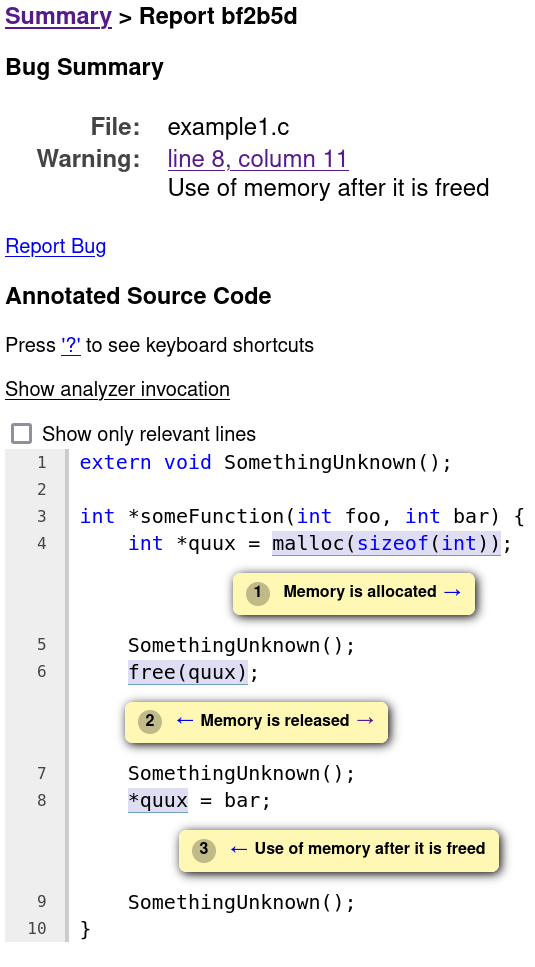
\includegraphics[height=0.9\textheight]{../static/scan-build-uaf-example1}
\end{frame}

\begin{frame}[fragile,label=useAfterFree2]{checking use-after-free (2)}
    \lstset{
        language=C,style=script,
        moredelim={**[is][\btHL<2>]{~2~}{~end~}},
    }
\begin{tikzpicture}
\node[anchor=north east] at (-.2, 0) {
\begin{lstlisting}
int *someFunction(int foo, int bar) {
    int *quux = malloc(sizeof(int));
    // A
    if (Complex(foo)) {
        free(quux);
        // B
    }
    ... /* omitted code that doesn't use quux */
    if (Complex(bar)) {
        // C
        *quux = bar;
    }
    ... /* omitted code that doesn't use quux */
    // D
}
\end{lstlisting}
};

    \tikzset{flow/.style={draw,thick,font=\fontsize{9}{10}\selectfont,anchor=north west},
    flowLine/.style={thick,-Latex}}
    \begin{scope}[y=0.8cm]
        \node[flow,dashed] (A) at (0, 0) { A: quux: \textit{allocated} };
        \begin{visibleenv}<2->
            \node[flow] (B) at (1, -1) { B: quux: \textit{freed} };
        \end{visibleenv}
        \begin{visibleenv}<3->
            \node[flow] (C1) at (1, -2) { C (from quux \textit{freed}): USE-AFTER-FREE };
        \end{visibleenv}
        \begin{visibleenv}<2->
            \node[flow] (D1) at (2, -3) { D (from quux \textit{freed})};
        \end{visibleenv}
        \begin{visibleenv}<4->
            \node[flow] (C2) at (1, -4) { C (from quux \textit{allocated}): ok };
            \node[flow] (D2) at (2, -5) { D (from allocated)};
        \end{visibleenv}
        \begin{visibleenv}<2->
            \draw[flowLine] ([xshift=.5cm]A.south west) |- ([yshift=.1cm]B.west);
        \end{visibleenv}
        \begin{visibleenv}<3->
            \draw[flowLine] ([yshift=-.1cm]B.west) -- ++(-.4cm, 0cm) |- ([yshift=.1cm]C1.west);
        \end{visibleenv}
        \begin{visibleenv}<2->
            \draw[flowLine] ([yshift=-.1cm]B.west) -- ++ (-.4cm,0cm) |- ([yshift=.1cm]D1.west);
        \end{visibleenv}
        \begin{visibleenv}<4->
            \draw[flowLine] ([xshift=.5cm]A.south west) |- ([yshift=.1cm]C2.west);
            \draw[flowLine] ([yshift=-.1cm]C2.west) -- ++(-.2cm,0cm) |- ([yshift=.1cm]D2.west);
            \draw[flowLine] ([xshift=.5cm]A.south west) |- ([yshift=.1cm]D2.west);
        \end{visibleenv}
    \end{scope}
    
    \begin{visibleenv}<4->
        \node[draw=red,very thick,fill=white,align=center,anchor=north west] at (-8, -6) {
            one idea: guess that Complex(foo) can be probably be true \\
            ~ \\
            option 1: say ``something wrong maybe''? \\
            option 2: try to figure out if Complex(foo) is true?)
        };
    \end{visibleenv}
\end{tikzpicture}
\end{frame}


\begin{frame}{result from clang's scan-build}
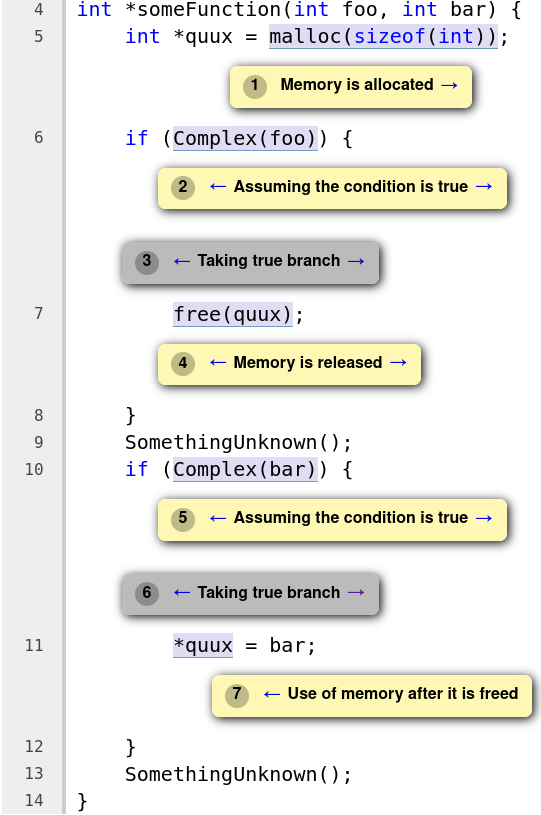
\includegraphics[height=0.9\textheight]{../static/scan-build-uaf-example2}
\end{frame}


    % FIXME: move loop discussion later

\subsection{exercise: aliasing and model}
\begin{frame}[fragile,label=homesModelExer]{exercise: holes in the model?}
\begin{tikzpicture}
\node (left) {
\begin{lstlisting}[language=C++,style=smaller]
void example(int a) {
    int *p;
    int *q;
    q = malloc(...);
    p = malloc(...);
    // (A)
    if (a > 0) {
        // (A1)
        p = q;
    }
    // (B)
    free(p);
    // (C)
    ...
}
\end{lstlisting}
};
\node[anchor=north west,align=left,draw,very thick] at (left.north east) {
exercise: what should state of pointer q be at C? \\
A. allocated \hspace{.5cm} B. freed \\
C. allocated if+only if reached via path with A1\\
D. freed if+only if reached via path with A1 \\
E. something else?
};
\end{tikzpicture}
\end{frame}

\begin{frame}{clang-analyzer output}
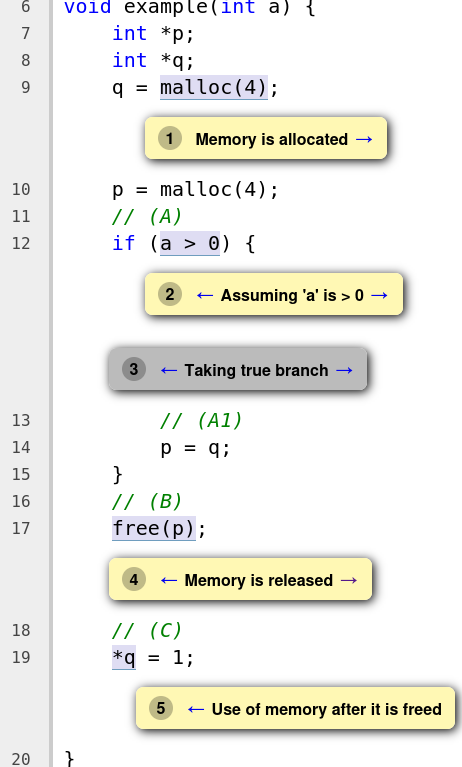
\includegraphics[height=0.9\textheight]{../static/clang-analyze-example4}
\end{frame}


\subsection{points-to analysis}
\usetikzlibrary{arrows.meta}

\begin{frame}{analysis building blocks}
    \begin{itemize}
    \item needed to track that \texttt{p} and \texttt{q} could point to same thing
    \vspace{.5cm}
    \item common prerequisite for all sorts of program analysis
    \end{itemize}
\end{frame}

\begin{frame}{overly simple algorithm for points-to analysis}
\begin{itemize}
\item for each pointer/reference track which objects it can refer to
\item if multiple paths: take union of all possible
\end{itemize}
\end{frame}

\begin{frame}[fragile,label=simplePointsTo]{simple points-to analysis}
\begin{lstlisting}[language=C++,style=smaller]
void example(int a) {
    int *p;
    int *q;
    q = malloc(...); // ID=1
    p = malloc(...); // ID=2
    // (A)
    if (a > 0) {
        p = q;
        // (B)
    }
    // (C)
    ...
}
\end{lstlisting}
\begin{tikzpicture}[overlay, remember picture]
    \tikzset{flow/.style={draw,thick,font=\fontsize{9}{10}\selectfont,anchor=north west,align=left},
    flowLine/.style={thick,-Latex}}
    \coordinate (base) at ([xshift=-9cm,yshift=-2cm]current page.north east);
    \begin{scope}[shift={(base)}]
        \begin{scope}
            \node[flow] (A) at (0, 0) { A: \myemph<2>{p (v1)}: \{ID=1\}; \myemph<2>{q (v1)}: \{ID=2\} };
            \node[flow] (B) at (1, -1) { B: \myemph<2>{p (v2)}: \{ID=2\}; \myemph<2>{q (v1)}: \{ID=2\} };
            \begin{visibleenv}<4->
            \node[flow] (C) at (0, -4) { C: \myemph<2>{p (v3)}: \myemph<3>{\{ID=1,ID=2\}}: \myemph<2>{q (v1)}: \{ID=2\} };
            \draw[flowLine] ([xshift=.5cm]A.south west) |- (B.west);
            \draw[flowLine] ([xshift=.5cm]B.south west) -- ([xshift=1.5cm]C.north west);
            \draw[flowLine] ([xshift=.5cm]A.south west) -- ([xshift=.5cm]C.north west);
            \end{visibleenv}
            \begin{visibleenv}<1-3>
            \node[flow] (C1) at (2, -2) { C via B: p (v2): \{ID=2\}: q (v1): \{ID=2\} };
            \node[flow] (C2) at (2, -3) { C not via B: p (v2): \{ID=1\}: q (v1): \{ID=2\} };
            \draw[flowLine] ([xshift=.5cm]A.south west) |- (B.west);
            \draw[flowLine] ([xshift=.5cm]B.south west) |- (C1.west);
            \draw[flowLine] ([xshift=.5cm]A.south west) |- (C2.west);
            \end{visibleenv}
        \end{scope}
        \begin{visibleenv}<2>
        \node[draw=red,very thick,align=left,font=\small] at (0, -6) {
            likely first step: mark different versions of p, q \\
            and track them as separate variables \\
            this way: can avoid storing set of values for q for every block of code \\
            (instead just point to q (v1) set)
        };
        \end{visibleenv}
        \begin{visibleenv}<4>
        \node[draw=red,very thick,align=left,font=\small] at (0, -6) {
            alternate idea: avoid path explosion by merging possible sets
        };
        \end{visibleenv}
        \begin{visibleenv}<3>
        \node[draw=red,very thick,align=left,font=\small] at (0, -6) {
            one idea: keep track of each path separately \\
            (but limit to how much one can do this)
        };
        \end{visibleenv}
    \end{scope}
\end{tikzpicture}
\end{frame}
 % FIXME: move earlier?

\subsection{complicating points-to analysis}
\begin{frame}{complicating points-to analysis}
    \begin{itemize}
    \item would like to analyze program function-at-a-time, but\ldots
        \begin{itemize}
        \item functions can change values shared by other functions
        \end{itemize}
    \item what about computed array indices?
    \item what about pointers to pointers?
    \item \ldots
    \vspace{.5cm}
    \item high false-positive solution:
        \begin{itemize}
        \item when incomplete info: assume value points to anything of right type
        \end{itemize}
    \item high false-negative solution:
        \begin{itemize}
        \item when incomplete info: assume value points to nothing
        \end{itemize}
    \end{itemize}
\end{frame}


\subsection{example: model for use-after-free, with loop}
\usetikzlibrary{arrows.meta}
\begin{frame}[fragile,label=useAfterFree3]{checking use-after-free (3)}
    \lstset{
        language=C,style=script,
        moredelim={**[is][\btHL<2>]{~2~}{~end~}},
    }
\begin{tikzpicture}
\node[anchor=north east] at (-.2, 0) {
\begin{lstlisting}
void someFunction() {
    int *quux = malloc(sizeof(int));
    ...
    // A
    do {
        // B
        ...
        if (anotherFunction()) {
            free(quux);
            // C
        }
        ...
        // D
    } while (complexFunction());
    ...
    // E
    *quux++;
    ...
}
\end{lstlisting}
};
    \tikzset{flow/.style={draw,thick,font=\fontsize{9}{10}\selectfont,anchor=north west},
    flowLine/.style={thick,-Latex},
    flowLineB/.style={very thick,dotted,-Latex},
    }
    \begin{scope}[y=0.8cm]
        \begin{visibleenv}<1->
        \node[flow] (A) at (0, 0) { A: \textit{allocated} };
        \node[flow,alt=<3>{red}{},alt=<1-2>{dashed}] (B) at (1, -1) { B (from \textit{allocated}): \textit{allocated} };
        \draw[flowLine] ([xshift=.5cm]A.south west) |- ([yshift=.1cm]B.west);
        \end{visibleenv}
        \begin{visibleenv}<2->
        \node[flow] (C1) at (1, -2) { C (from \textit{allocated}): quux: \textit{freed} };
            \node[flow,alt=<1-4>{dashed}{}] (D1) at (1, -3) { D (from \textit{freed}): \textit{freed} };
        \node[flow] (E1) at (2, -4) { E (from \textit{freed}): USE-AFTER-FREE };
        \draw[flowLine] ([yshift=-.1cm]B.west) -- ++(-.2cm, 0cm) |- ([yshift=.1cm]C1.west);
        \draw[flowLine] ([yshift=-.1cm]C1.west) -- ++(-.2cm, 0cm) |- ([yshift=.1cm]D1.west);
        \draw[flowLine] ([yshift=-.1cm]D1.west) -- ++(-.2cm, 0cm) |- ([yshift=.1cm]E1.west);
        \end{visibleenv}
        \begin{visibleenv}<3->
        \node[flow,alt=<3>{dashed}{}] (D2) at (1, -5) { D (from \textit{allocated}): \textit{allocated} };
        \draw[flowLine,alt=<3>{red}{}] ([yshift=-.1cm]B.west) -- ++(-.3cm, 0cm) |- ([yshift=.1cm]D2.west);
        \node[flow] (E2) at (2, -6) { E (from \textit{allocated}): ok };
        \draw[flowLine,alt=<3>{red}{}] ([yshift=-.1cm]D2.west) -- ++(-.2cm, 0cm) |- ([yshift=.1cm]E2.west);
        \end{visibleenv} 
        \begin{visibleenv}<4->
        \draw[flowLineB,alt=<4>{red}{}] ([yshift=-.1cm]D2.east) -- ++(2.5cm, 0cm) |- ([yshift=.1cm]B.east);
        \end{visibleenv} 
        \begin{visibleenv}<5->
            \node[flow,alt=<5>{dashed}{}] (B2) at (1, -7) { B (from \textit{freed}): \textit{freed} };
            \draw[flowLine,alt=<5>{red}{}] ([yshift=-.1cm]D1.west) -- ++(-.8cm, 0cm) |- ([yshift=.1cm]B2.west);
            \node[flow] (C2) at (1, -8) { C (from \textit{freed}): DOUBLE-FREE };
            \draw[flowLine] ([yshift=-.1cm]B2.west) -- ++(-.8cm, 0cm) |- ([yshift=.1cm]C2.west);
        \end{visibleenv} 
        \begin{visibleenv}<6->
            \draw[flowLineB,alt=<6>{red}{}] ([yshift=-.1cm]B2.east) -- ++(3cm, 0cm) |- ([yshift=.2cm]D1.east);
        \end{visibleenv}
    \end{scope}
\end{tikzpicture}
\end{frame}

\begin{frame}{result from clang's scan-build}
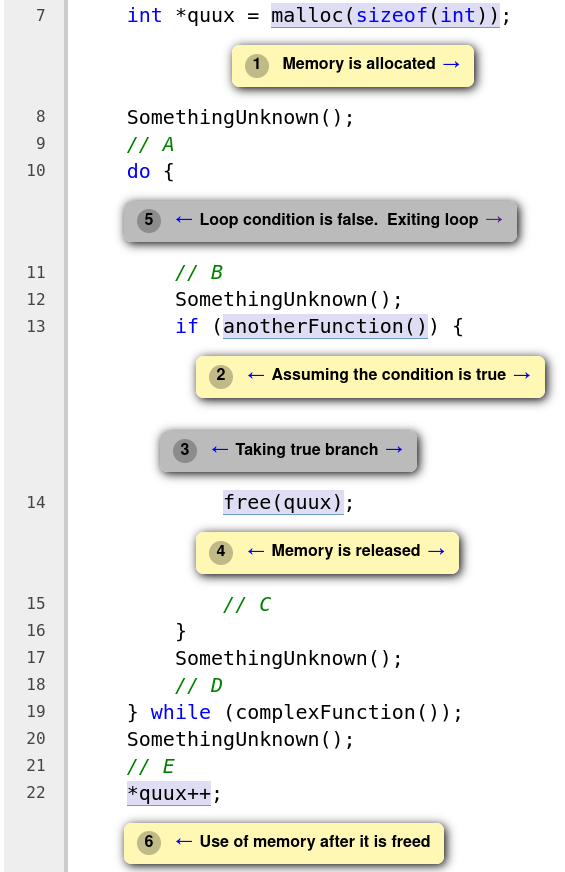
\includegraphics[height=0.9\textheight]{../static/scan-build-uaf-example3a}
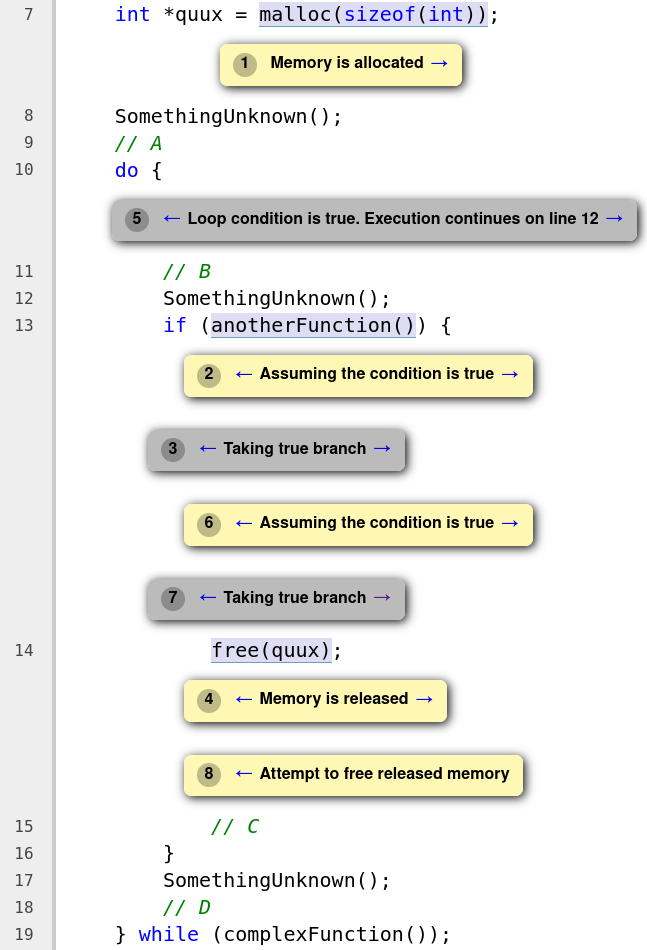
\includegraphics[height=0.9\textheight]{../static/scan-build-uaf-example3b}
\end{frame}


\subsection{example: model for array bounds}
\usetikzlibrary{arrows.meta}
\begin{frame}{checking for array bounds}
    \begin{itemize}
    \item can \textit{try} to apply same technique to array bounds
    \item but much more complicated/more likely to have false positives/negatives
    \vspace{.5cm}
    \item for each array or pointer track:  
        \begin{itemize}
        \item minimum number of elements before/after what it points to
        \end{itemize}
    \item for each integer track: 
        \begin{itemize}
        \item minimum bound
        \item maximum bound
        \end{itemize}
    \item similar analysis looking at paths?
    \end{itemize}
\end{frame}

\begin{frame}[fragile,label=bounds1]{checking array bounds (1)}
    \lstset{
        language=C,style=script,
        moredelim={**[is][\btHL<2>]{~2~}{~end~}},
    }
\begin{tikzpicture}
\node[anchor=north east] at (-.2, 0) {
\begin{lstlisting}
int array[100];
void someFunction(int foo) {
    // A
    if (foo > 100) {
        return;
    }
    // B
    array[foo] += 1;
}
\end{lstlisting}
};

    \tikzset{
        flow/.style={draw,thick,font=\fontsize{9}{10}\selectfont,anchor=north west},
        flowLine/.style={thick,-Latex},
    }
    \begin{scope}[y=1.2cm]
        \node[flow] (A) at (0, 0) { A: foo: $[-\inf, +\inf]$; array: indices [0, 99] };
        \node[flow] (B) at (0, -1) { B: foo: $[-\inf, +100]$; array: indices [0, 99] };
        \draw[flowLine] (A) -- (B);
    
    \begin{visibleenv}<2->
        \node[draw=red,very thick,fill=white,align=center] at (0, -4) {
            give warning about \texttt{foo == 100}? probably bug! \\
            give warning about \texttt{foo < 0}? maybe??
        };
    \end{visibleenv}
    \end{scope}
\end{tikzpicture}
\end{frame}

\begin{frame}[fragile,label=bounds2]{checking array bounds (2)}
    \lstset{
        language=C,style=script,
        moredelim={**[is][\btHL<2>]{~2~}{~end~}},
    }
\begin{tikzpicture}
\node[anchor=north east] at (-.2, 0) {
\begin{lstlisting}
int array[100];
void someFunction(int foo, bool bar) {
    int *p = array;
    // A
    p += 50;
    // B
    if (foo >= 50 || foo < 0) abort();
    // C
    if (bar) {
        foo = -foo;
    }
    // D
    p[foo] = 1;
}
\end{lstlisting}
};

    \tikzset{flow/.style={draw,thick,font=\fontsize{9}{10}\selectfont,anchor=north west},
    flowLine/.style={thick,-Latex}}
    \begin{scope}[y=1.2cm]
        \node[flow] (A) at (0, 0) { A: p: indices [0, 99]; foo: $[-\inf, +\inf]$ };
        \node[flow] (B) at (0, -1) { B: p: indices [-50, 49]; foo: $[-\inf, +\inf]$ };
        \node[flow] (C) at (0, -2) { C: p: indices [-50, 49]; foo: [0, 50] };
        \node[flow] (D1) at (-4, -3) { D (bar true): p: indices: [-50, 49]; foo: [-50, 0] } ;
        \node[flow,alt=<2>{draw=red}] (D2) at (1, -4) { D (bar false): p: indices: [-50, 49]; foo: [0, 50] };
        \draw[flowLine] (A) -- (B);
        \draw[flowLine] (B) -- (C);
        \draw[flowLine] (C) -- (D1);
        \draw[flowLine] (C) -- (D2);
    
    \begin{visibleenv}<2->
        \node[draw=red,very thick,fill=white,align=center] at (0, -6) {
            warn about possible out-of-bounds? 
        };
    \end{visibleenv}
    \end{scope}
\end{tikzpicture}
\end{frame}


\subsection{analysis for common insecure patterns}
\begin{frame}{common bug patterns}
    \begin{itemize}
    \item effectively detecting things like ``arrays are in bounds'' \\
        or ``values aren't used after being freed'' \\
        is not very reliable for large programs
    \item (but analysis tools are getting better)
    \vspace{.5cm}
    \item but static analysis tools shine for \myemph{common bug patterns}
    \end{itemize}
\end{frame}

\begin{frame}[fragile,label=suspectPatterns]{patterns clang's analyzer knows}
\begin{lstlisting}[language=C,style=smaller]
struct foo *p = malloc(sizeof(struct foo*)); // meant struct foo?
long *p = malloc(16 * sizeof(int)); // meant sizeof(long)?
\end{lstlisting}
\hrule
\begin{lstlisting}[language=C,style=smaller]
strncat(foo, bar, sizeof(foo));
\end{lstlisting}
\hrule
\begin{lstlisting}[language=C,style=smaller]
int *global;
int *foo() {
    int x;
    int *p = &x;
    ...
    global = p; // putting pointer to stack in global
    return p;    // returning pointer to stack
}
\end{lstlisting}
\end{frame}

\begin{frame}[fragile,label=suspectPatterns]{more suspect patterns }
    \begin{itemize}
    \item SpotBugs: Java static analysis tool
    \end{itemize}
\begin{lstlisting}[language=Java,style=smaller]
// pattern: connecting to database with empty password:
connection = DriverManager.getConnection(
    "jdbc:hsqldb:hsql://db.example.com/xdb" /* database ID */, 
    "sa" /* username */, "" /* password */);

// pattern: Sql.hasResult()'s second argument isn't a constant
Sql.hasResult(c, "SELECT 1 FROM myTable WHERE code='"+code+"'");

// pattern: new FileReader's argument comes from request
HttpRequest request = ...;
String path = request.getParameter("path");
BufferedReader r = new BufferedReader(
    new FileReader("data/" + path));
\end{lstlisting}
\end{frame}


\subsection{static analysis limits?}
\begin{frame}{static analysis}
    \begin{itemize}
    \item need to avoid exploring way too many paths
        \begin{itemize}
        \item clang-analyzer: only a procedure at a time
        \item other analyzers: some way of pruning paths
        \end{itemize}
    \item need to avoid false positives
        \begin{itemize}
        \item probably can't always assume every if can be true/false
        \item one idea: apply symbolic-execution like techniques to prune
        \item clang-analyzer: limited by being procedure-at-a-time
        \end{itemize}
    \end{itemize}
\end{frame}


\begin{frame}{preview: information flow}
    \begin{itemize}
    \item really common pattern we want to find: \\
        data from somewhere gets to dangerous place
        \begin{itemize}
        \item pointer to stack escapes function
        \item input makes it to SQL query, file name
        \end{itemize}
    \item we'll talk about it specially next
    \end{itemize}
\end{frame}

\subsection{summary / actual tools}
\begin{frame}[fragile,label=practic]{static analysis practicality}
    \begin{itemize}
    \item good at finding some kinds of bugs
        \begin{itemize}
        \item array out-of-bounds probably not one --- complicated tracking needed
        \end{itemize}
    \item excellent for ``bug patterns'' like:
\begin{lstlisting}
struct Foo* foo;
...
foo = malloc(sizeof(struct Bar));
\end{lstlisting}
    \item false positive rates are often 20+\% or more
    \item some tools assume lots of annotations
    \item not limited to C-like languages
    \end{itemize}
\end{frame}

\begin{frame}{static analysis tools}
    \begin{itemize}
    \item Coverity, Fortify --- commerical static analysis tools
    \item Splint --- unmaintained?
        \begin{itemize}
            \item written by David Evans and his research group in the late 90s/early 00s
        \end{itemize}
    \item FindBugs (Java)
    \item clang-analyzer --- part of Clang compiler
    \item Microsoft's Static Driver Verifier  --- required for Windows drivers:
        \begin{itemize}
            \item mostly checks correct usage of Windows APIs
        \end{itemize}
    \end{itemize}
\end{frame}



\end{document}
